\chapter{Results}
\label{ch:chapter5}

My  

\section{Platform and Software}
\label{sub:platform-software}
I ran the \OpenMC simulation on Sawtooth, a supercomputer at
\Gls{inl}. On Sawtooth, the compute nodes have 2 Intel Xeon 8268 CPUs with 24 cores per
CPU. Hyper-threading is disabled on compute nodes. Each node has 192 GB of RAM.
The login nodes have the same specifications. See Table \ref{tab:sawtooth-params}
for the full specifications of the machine. To avoid any potential licensing
issues with getting \SerpentTWO on Sawtooth, I performed the \SerpentTWO runs
on my office computer, a Dell Precision 3430 Workstation, using 12 OpenMP threads.

\begin{table}[htpb] 
    \centering 
    \caption{Sawtooth job parameters for 100k particle \OpenMC run}
    \label{tab:sawtooth-params}
    \begin{tabular}{|c|c|} 
        \hline
        Quantity & Value\\
        \hline
        Nodes & 92 \\
        \hline
        MPI processes per node & 6 \\
        \hline
        Threads per core & 1 \\
        \hline
        OpenMP threads per MPI process & 8 \\
        \hline
    \end{tabular}
\end{table}
% make this subsection a table

\subsection{Simulation Design and Parameters}
\label{sub:simulation-parameters}

The purpose of these simulations is to test the accuracy of
the implementation of \OpenMC support, so we do not need to do as detailed an
analysis as Ryhlevskii did on finding the equilibrium state. A moderate amount
of timesteps will suffice. I decided to use the same 3 day timesteps as Ryhklevskii
\cite{rykhlevskii_modeling_2019} (as discussed in Section \ref{sub:reprocessing-system-model})
for a year's worth of runtime. Table \ref{tab:saltproc-params} summarizes the simulation
settings used for both the \SerpentTWO and \OpenMC simulations. While I had intended
to use interpolated fission product yields for both the \OpenMC and \SerpentTWO simulations,
I realized very late into the process of writing this manuscript that I had forgotten to set
that option in \OpenMC. This may be one of the reasons some results have larger errors than expected.
 
\begin{table}[htpb] 
    \centering 
    \caption{Neutronics and Depletion parameters for \SaltProc}
    \label{tab:saltproc-params}
    \begin{tabular}{|c|c|} 
        \hline
        Batches & 200 \\
        \hline
        Inactive batches & 80 \\
        \hline
        Particles per batch & 1e6 \\
        \hline
        Power [W] & 2.25e9 \\
        \hline
        Depletion steps & 122 \\
        \hline
        Depletion step length [days] & 3 \\
        \hline
        Depletion equation solver & IPF CRAM 48 \\
        \hline
        Time integration method & Euler's Method \\
        \hline
    \end{tabular}
\end{table}

\subsection{Data}
\label{sub:results-xs-data}

I used neutron reaction cross sections from the {\bf endf71x} \cite{conlin_continuous_2013} library and
thermal scattering cross sections {\bf ENDF70SaB} \cite{trellue_release_2008} library
for both the \SerpentTWO and \OpenMC simulations. While the
{\bf endf71x} library is based on the evaluated neutron reaction data from the ENDF/B-VII.1 library \cite{chadwick_endf/b-vii.1_2011},
the {\bf ENDF70SaB} library is based on evaluated thermal scattering data from the ENDF/B-VII.0 library \cite{chadwick_endfb-vii0_2006}.
Fortunately, the thermal scattering data in the ENDF/B-VII.0 library is the same as the same thermal
scattering data as the ENDF/B-VII.1 library, with the primary difference being that the thermal
neutron scattering data in ENDF/B-VII.1 uses a continuous representation
that \SerpentTWO v2.1.32 does not support.

To ensure data consistency, I downloaded the \verb,.ace, files from the \Gls{lanl}
website, then processed these files into HDF5 format using the \OpenMC Python
API. I also used the Python API to create a depletion chain from the
spontaneous and delayed fission yield data, decay data, and neutron cross
section data from the ENDF B/VII.1 library\footnote{Interested readers are able to
create this library files by running the scripts located at
\url{https://github.com/arfc/saltproc/tree/master/scripts/xsdata}. See
the README.md in the parent directory for user instructions}.

As discussed in Section \ref{sub:msbr-fuel-salt}, the average temperature of the
fuel between the core inlet and outlets is around 900K, and this is the value I used
for all material temperatures. For cross section data
unavailable at that temperature, I used interpolation between 800K and 1000
to get reasonable values for the cross sections.

\section{Comparison of OpenMC to Serpent}
\label{sec:openmc-vs-serpent}

\begin{figure}[htpb]
    \centering
    \subfloat[][]{
        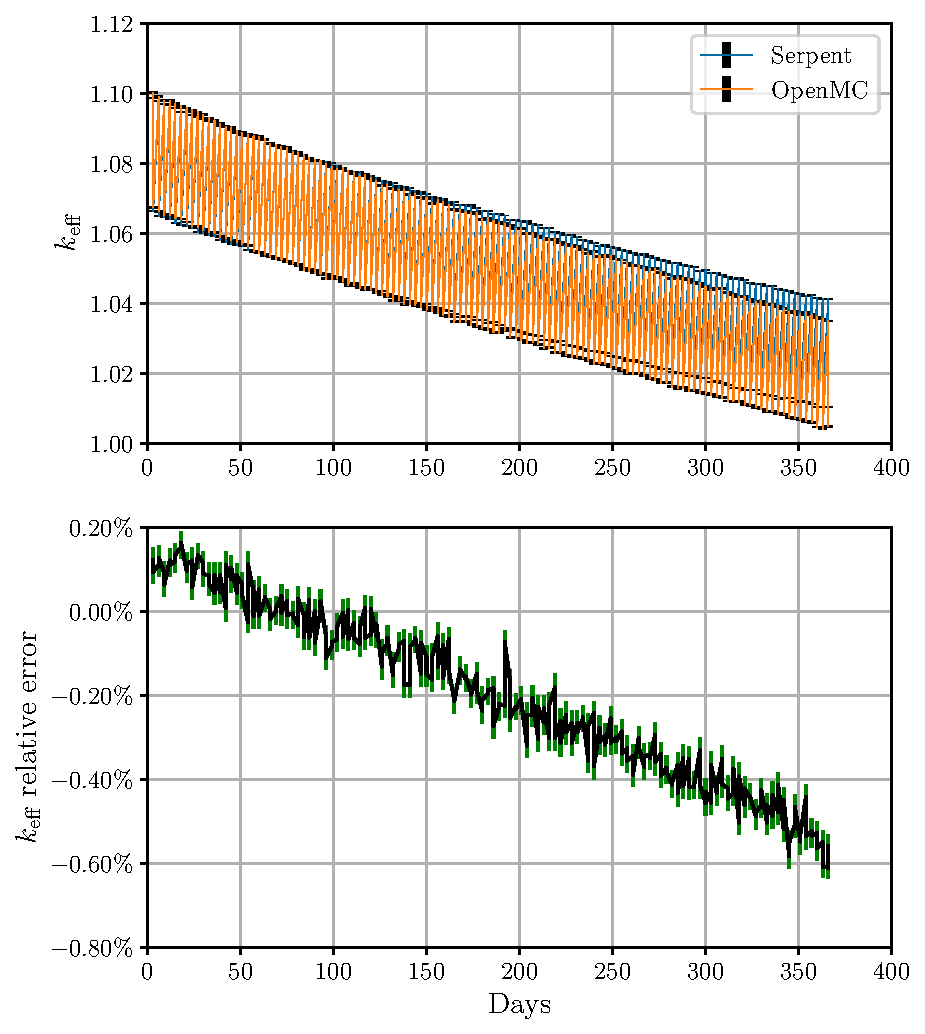
\includegraphics[width=0.8\linewidth]{figs/ch5/keff.pdf}
        \label{fig:keff}

    }\\
    \subfloat[][]{
        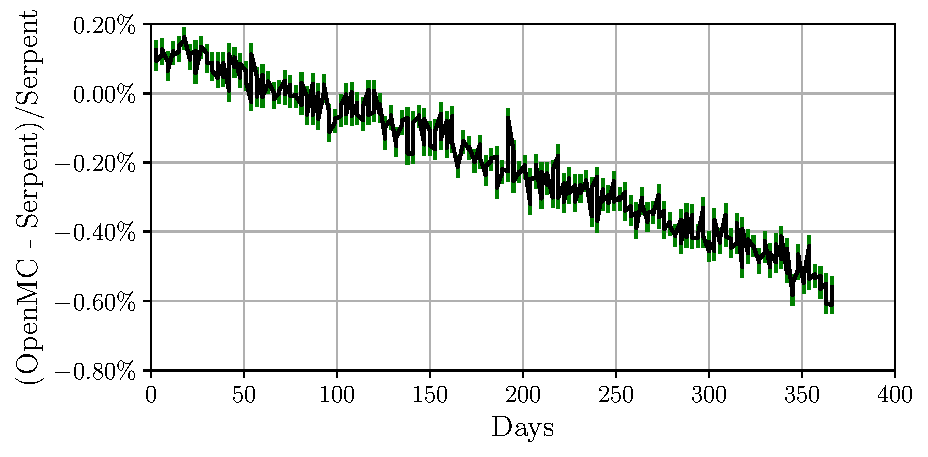
\includegraphics[width=0.8\linewidth]{figs/ch5/keff_error.pdf}
        \label{fig:keff_err}
    }
    \caption[$k_\text{eff}$ difference between \OpenMC and \SerpentTWO over time]{
        \subref{fig:keff} $k_\text{eff}$ difference between \OpenMC and \SerpentTWO over time;
        \subref{fig:keff_err} $k_\text{eff}$ relative difference between \OpenMC and \SerpentTWO 
        over time.
    }
    \label{fig:keff_sum}
\end{figure}

Figure \ref{fig:keff_sum} shows the change in $k_\text{eff}$ over time in the \OpenMC and \SerpentTWO
coupled simulations, as well as the relative difference between.
In Figure \ref{fig:keff}. the error bars are black, and in Figure
\ref{fig:keff_err}, they are green. For the first 70 days or so, the
$k_\text{eff}$ calculated by \OpenMC is slightly  higher than the 
$k_\text{eff}$ calculated by \SerpentTWO, with a difference of around 150 pcm.
After 70 days, the $k_\text{eff}$ calculated by \OpenMC is becomes smaller than
the $k_\text{eff}$ calculated by \SerpentTWO. As time goes on, the difference
between the two grows constantly. At the end of the simulation, the absolute
value of the relative difference is around 0.6\%, or 600 pcm. Notice the
oscillating behavior of $k_\text{eff}$. This is due to fuel reprocessing every 3 days.

% If we did not reprocess the fuel, the simulation
%would look like \ldots

\subsection{Nuclide compositions}
\label{sub:nuclide-compositions}

\begin{figure}[htpb]
    \centering
    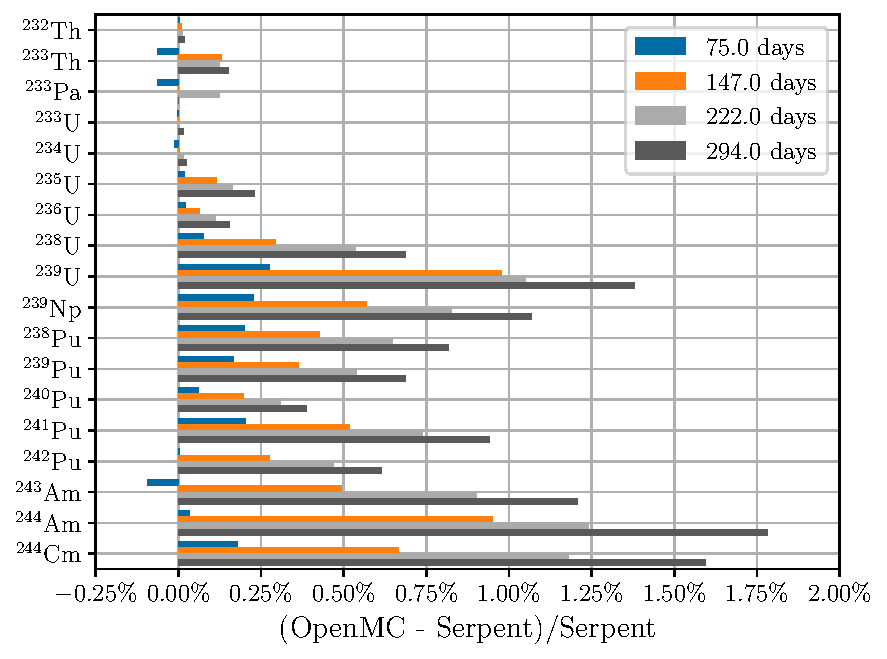
\includegraphics[width=0.8\textwidth]{figs/ch5/actinides.pdf}
    \caption[Relative difference of actinides mass in fuel at selected time steps]{Relative difference of actinides mass between \OpenMC and \SerpentTWO
    coupled simulations at 75, 147, 222, and 294 days. \ce{^{242m}Am}, \ce{^{242}Cm},
    \ce{^{245}Cm}, \ce{^{246}Cm} have been ommited here due to their high difference,
    and can be found in Figures \ref{fig:am242m-mass}, \ref{fig:cm242-mass},
    \ref{fig:cm245-mass}, and \ref{fig:cm246-mass}, resepectively.
    \label{fig:actinides}
\end{figure}

Figure \ref{fig:actinides} shows the relative error of actinide mass in the fuel
salt at several points in the simulation. As time goes on, the error for
\ce{^{241}Am}, \ce{^{242}Am}, and \ce{^{235}U} generally decreases in
magnitude, and for the rest of the actinides it increases in magnitude. The
maximum error for the actinides is around 8\% at the end of the simulation.

The main fissionable nuclide in our fuel salt is \ce{^{233}U}, and the
composition in the \OpenMC fuel is less than the composition in the \SerpentTWO
fuel. This is consistent with our results for $k_\text{eff}$.

\begin{figure}[htpb]
    \centering
    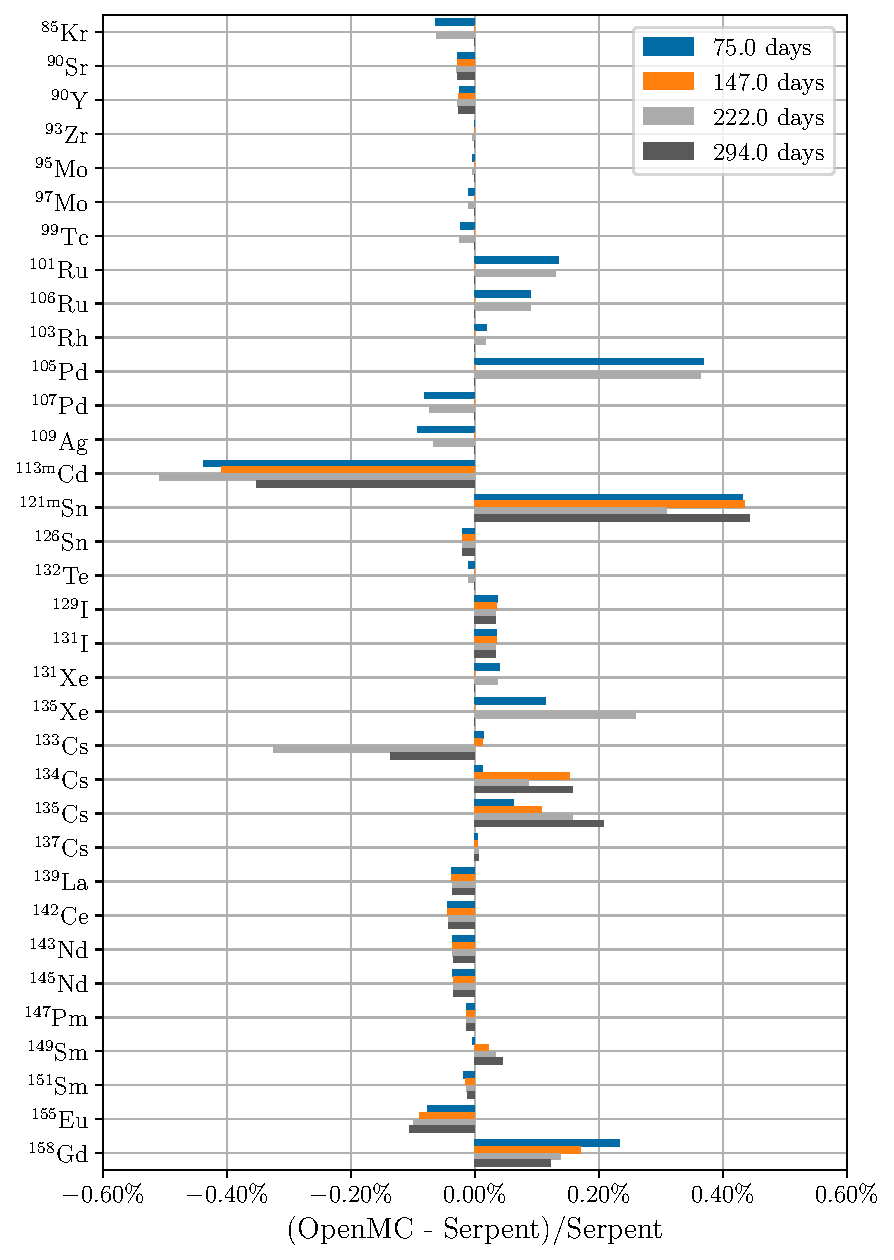
\includegraphics[width=0.8\textwidth]{figs/ch5/fission_products.pdf}
    \caption{Relative error of fission products mass in fuel. \ce{^{97}Mo}
        has been omitted to
        maintain clarity in the results. It's error is around -20\%
    }
    \label{fig:fission-products}
\end{figure}

Figure \ref{fig:fission-products} shows the relative error of fission product
mass in the fuel. The behavior of the error varies depending on the nuclide.
The maximum error for the fission products that are not cesium is around 3\%
and the end of the simulation.

%go into detail about each nuclide?

\ce{^{242}Cm} is one of the few actinides with significant error early in the
simulation that even out later on. Figure \ref{fig:cm242-mass} shows this
behavior

\begin{figure}[htpb]
    \centering
    \subfloat[][]{
        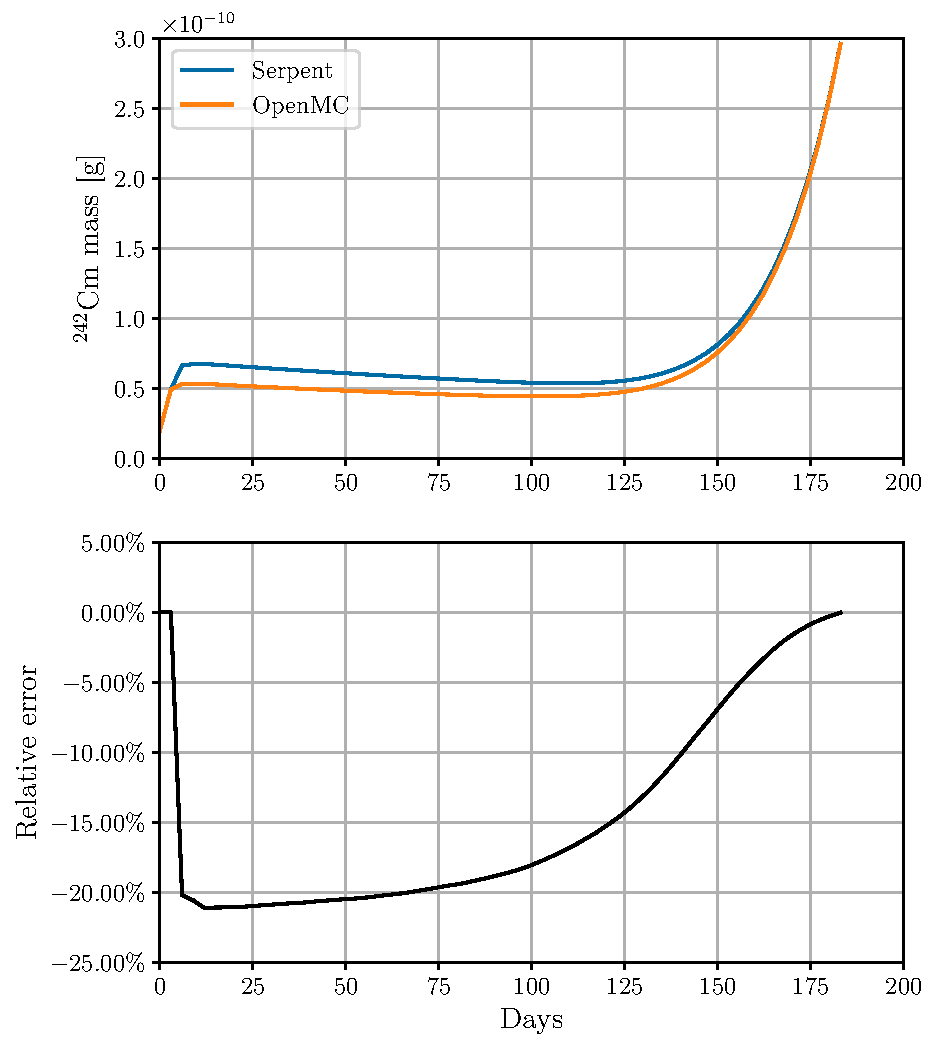
\includegraphics[width=0.5\linewidth]{figs/ch5/Cm242_mass_0.pdf}
        \label{fig:cm242-mass-0}
    }
    \subfloat[][]{
        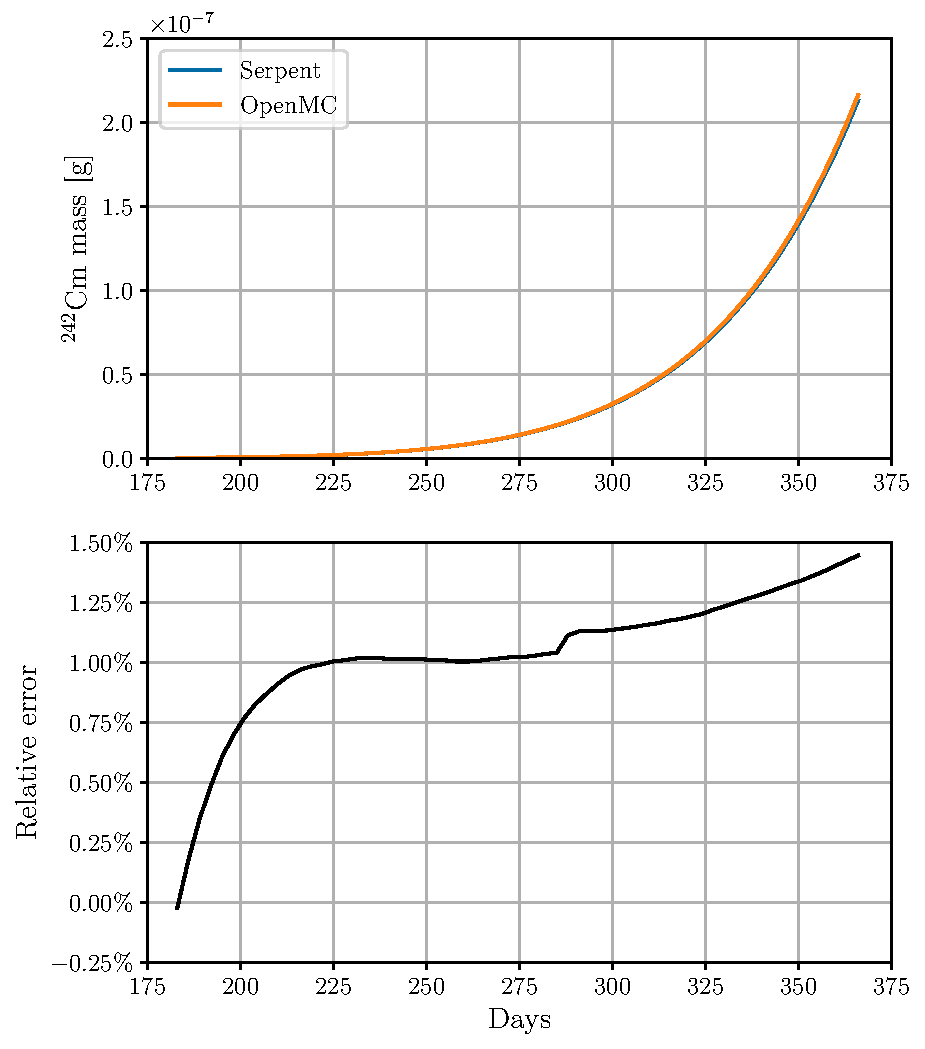
\includegraphics[width=0.5\linewidth]{figs/ch5/Cm242_mass_1.pdf}
        \label{fig:cm242-mass-1}
    }
    \caption{}
    \caption[\ce{^{242}Cm} mass]{
    \subref{fig:cm242-mass-0} \ce{^{242}Cm} mass up to 183 days;
    \subref{fig:cm242-mass-1} \ce{^{242}Cm} mass after 183 days}
    \label{fig:cm242-mass}
\end{figure}

There are several important actinides, that
have very large errors for all but the first depletion step, specifically
\ce{^{242m}Am}, \ce{^{245}Cm}, and  \ce{^{246}Cm}. Figures
\ref{fig:am242_m1-mass}, \ref{fig:cm245-mass}, and \ref{fig:cm246-mass} show
the behavior for each of these nuclides, respectively.

\begin{figure}[htpb]
    \centering
    \subfloat[][]{
        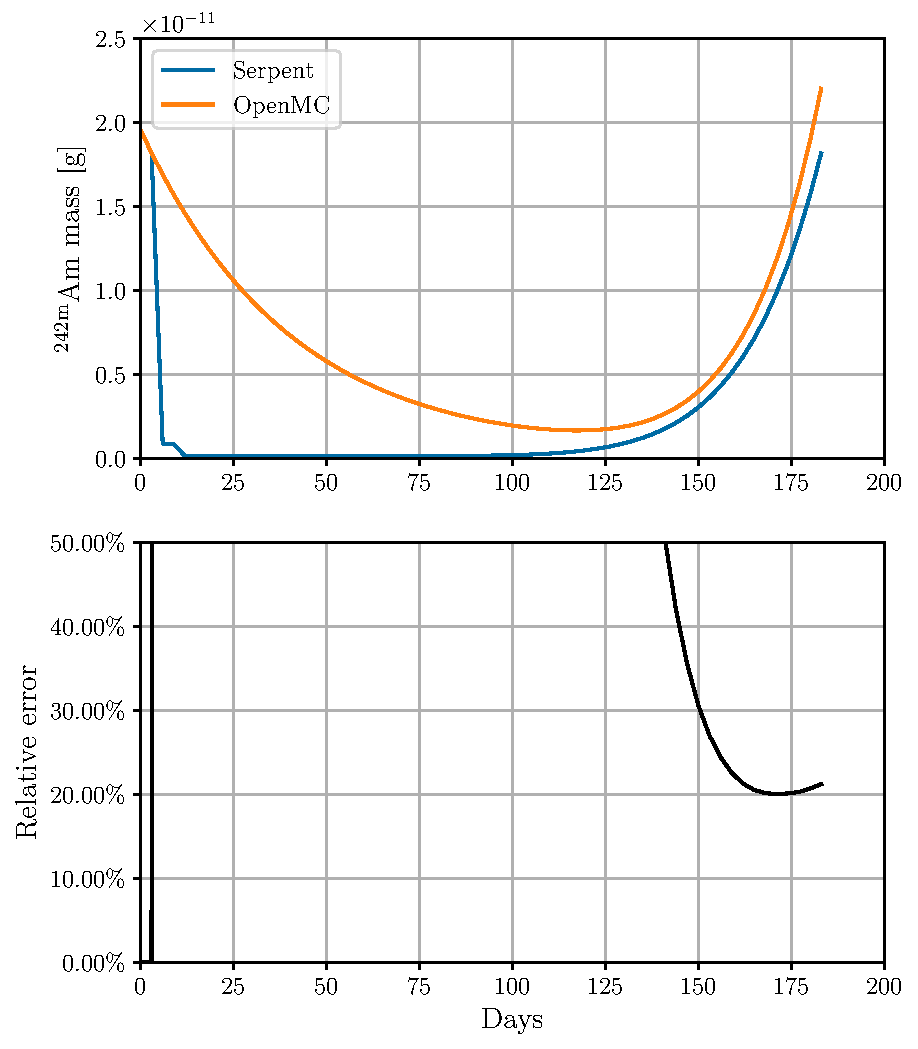
\includegraphics[width=0.5\linewidth]{figs/ch5/Am242_m1_mass_0.pdf}
        \label{fig:am242_m1-mass-0}
    }
    \subfloat[][]{
        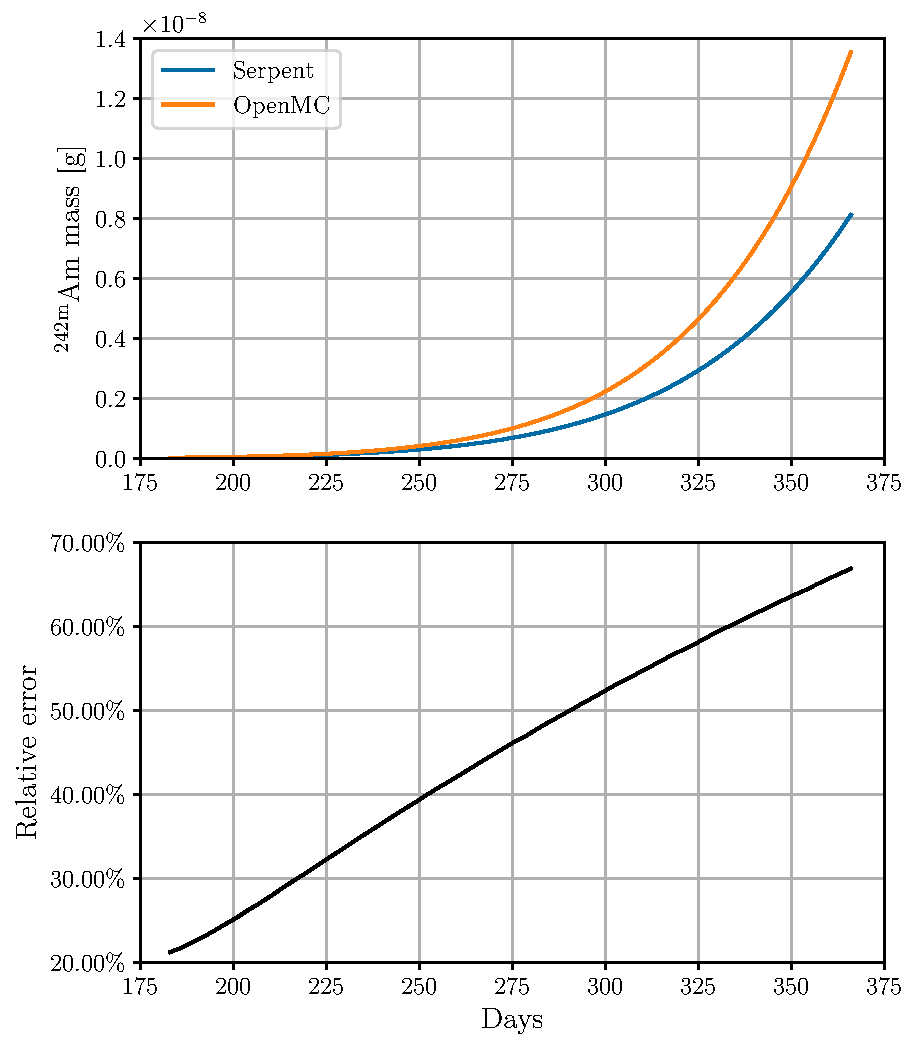
\includegraphics[width=0.5\linewidth]{figs/ch5/Am242_m1_mass_1.pdf}
        \label{fig:am242_m1-mass-1}
    }
    \caption[\ce{^{242m}Am} mass]{
    \subref{fig:am242_m1-mass-0} \ce{^{242m}Am} mass up to 183 days;
    \subref{fig:am242_m1-mass-1} \ce{^{242m}Am} mass after 183 days}
    \label{fig:am242_m1-mass}
\end{figure}

\begin{figure}[htpb]
    \centering
    \subfloat[][]{
        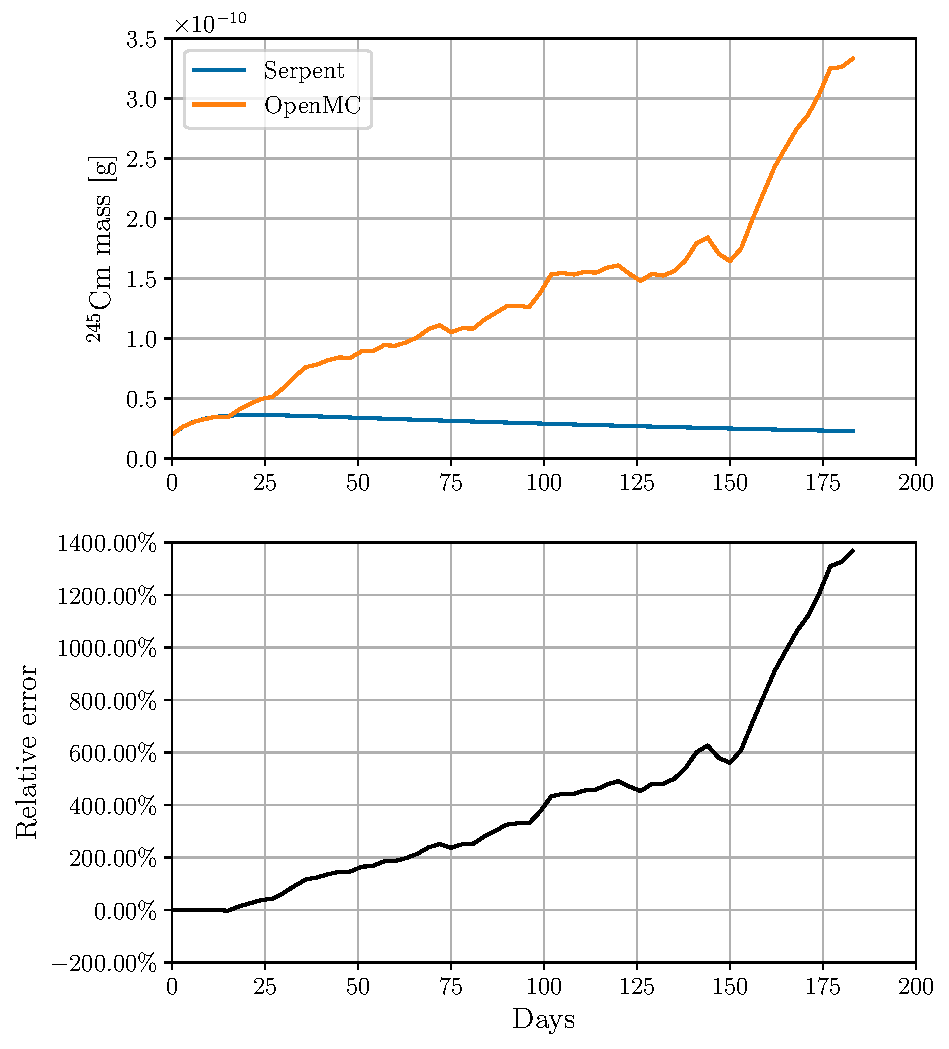
\includegraphics[width=0.5\linewidth]{figs/ch5/Cm245_mass_0.pdf}
        \label{fig:cm245-mass-0}
    }
    \subfloat[][]{
        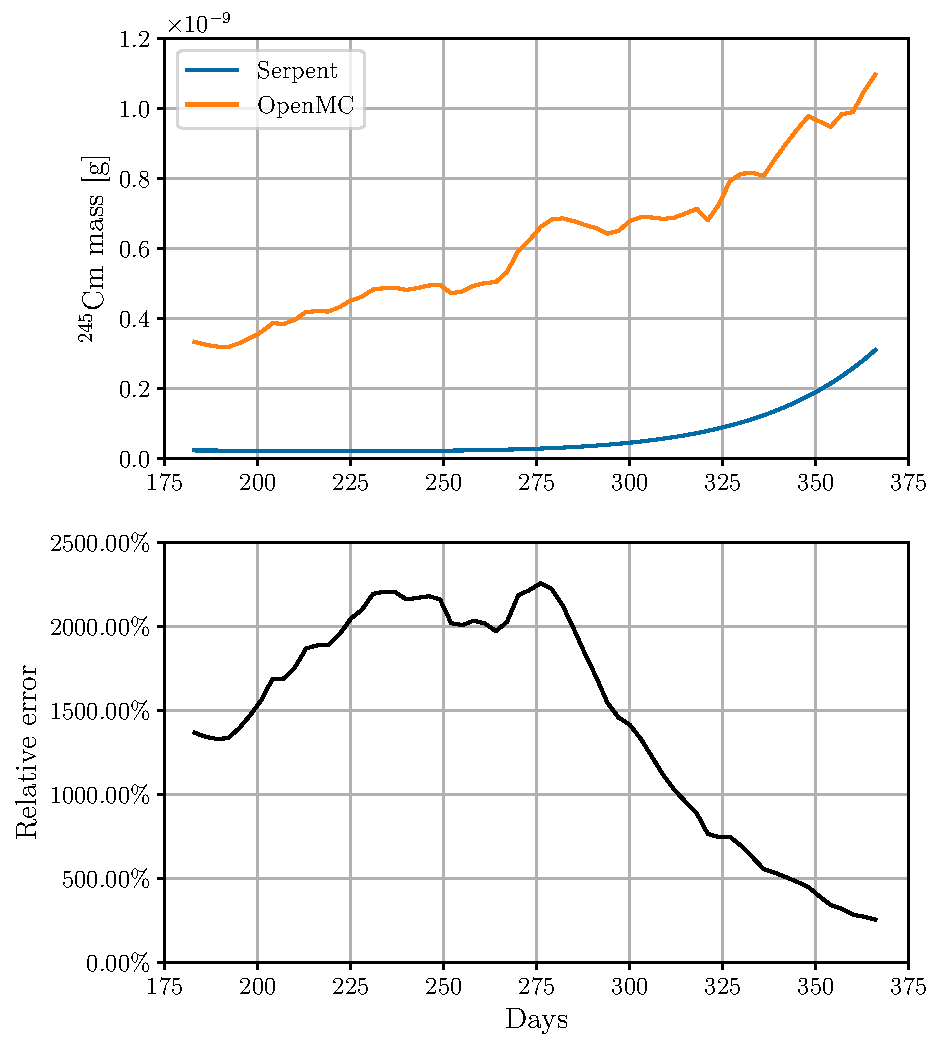
\includegraphics[width=0.5\linewidth]{figs/ch5/Cm245_mass_1.pdf}
        \label{fig:cm245-mass-1}
    }
    \caption{}
    \caption[\ce{^{245}Cm} mass]{
    \subref{fig:cm245-mass-0} \ce{^{245}Cm} mass up to 183 days;
    \subref{fig:cm245-mass-1} \ce{^{245}Cm} mass after 183 days}
    \label{fig:cm245-mass}
\end{figure}

\begin{figure}[htpb]
    \centering
    \subfloat[][]{
        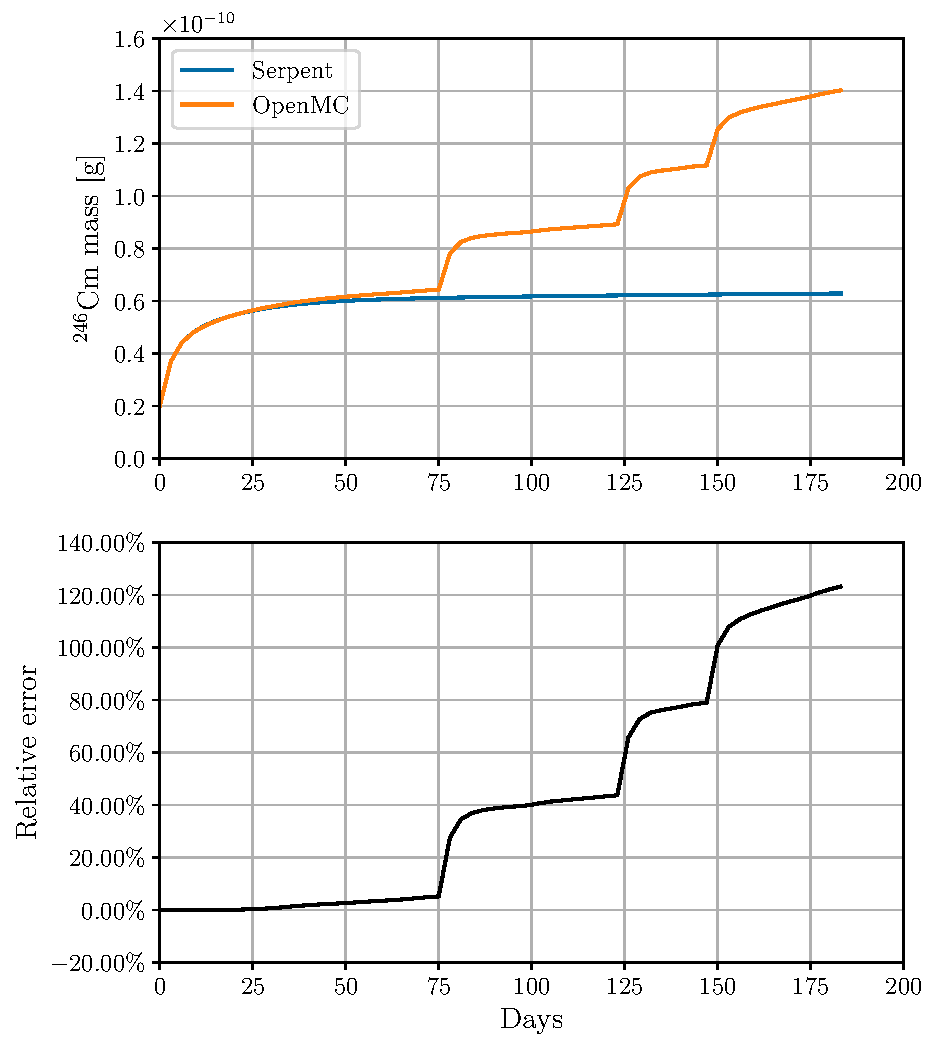
\includegraphics[width=0.5\linewidth]{figs/ch5/Cm246_mass_0.pdf}
        \label{fig:cm246-mass-0}
    }
    \subfloat[][]{
        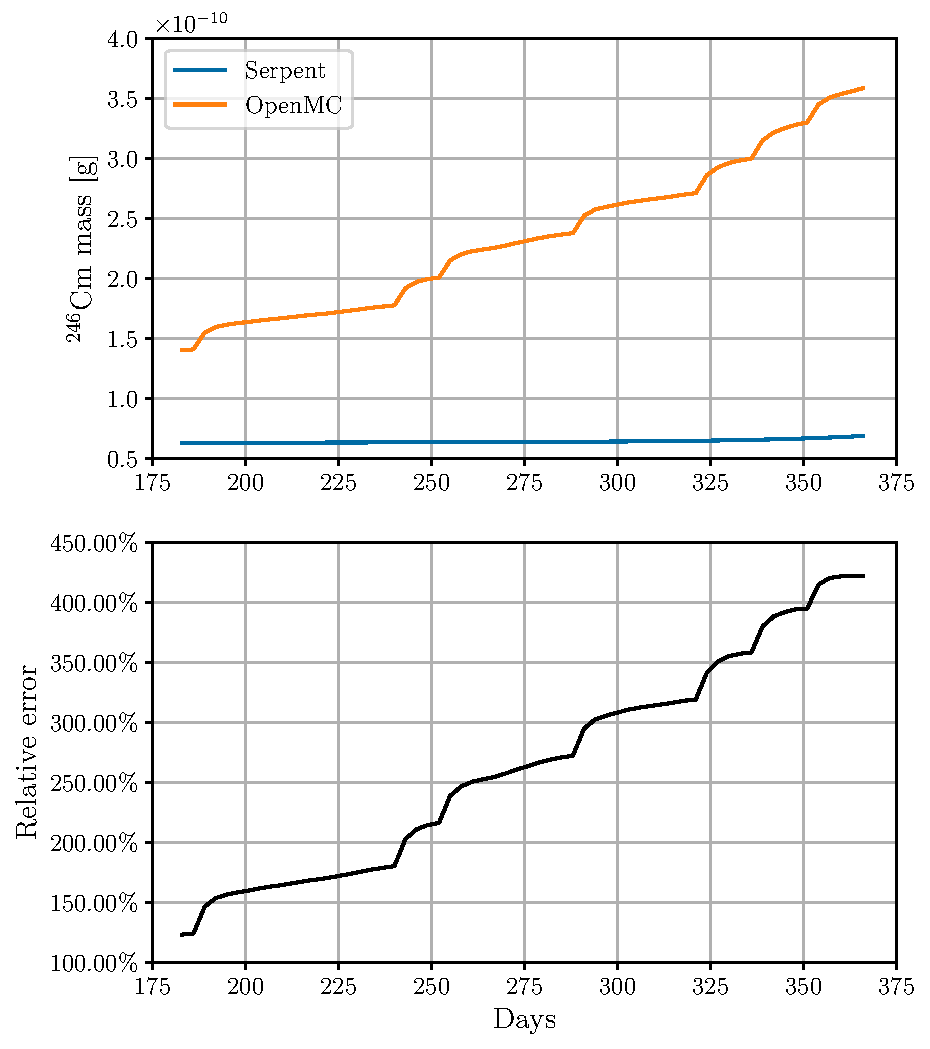
\includegraphics[width=0.5\linewidth]{figs/ch5/Cm246_mass_1.pdf}
        \label{fig:cm246-mass-1}
    }
    \caption{}
    \caption[\ce{^{246}Cm} mass]{
    \subref{fig:cm246-mass-0} \ce{^{246}Cm} mass up to 183 days;
    \subref{fig:cm246-mass-1} \ce{^{246}Cm} mass after 183 days}
    \label{fig:cm246-mass}
\end{figure}


From a computational perspective, the high errors after the first timestep may
be due to the extremely small amount of these nuclides present in the material.
This would not effect the first depletion step, as the materials for both
simulations have been verified to be using the same initial compositions.
However, due to the control flow described in section
\ref{sec:saltproc-detail}, the nuclide compositions of nuclides present in
small amounts could be effected.

%\subsection{Elements targeted for removal}
%\label{sub:removed-elements}
